\documentclass[tikz,border=8pt]{standalone}
\usepackage{amsmath}
\usetikzlibrary{arrows.meta,positioning}

\begin{document}
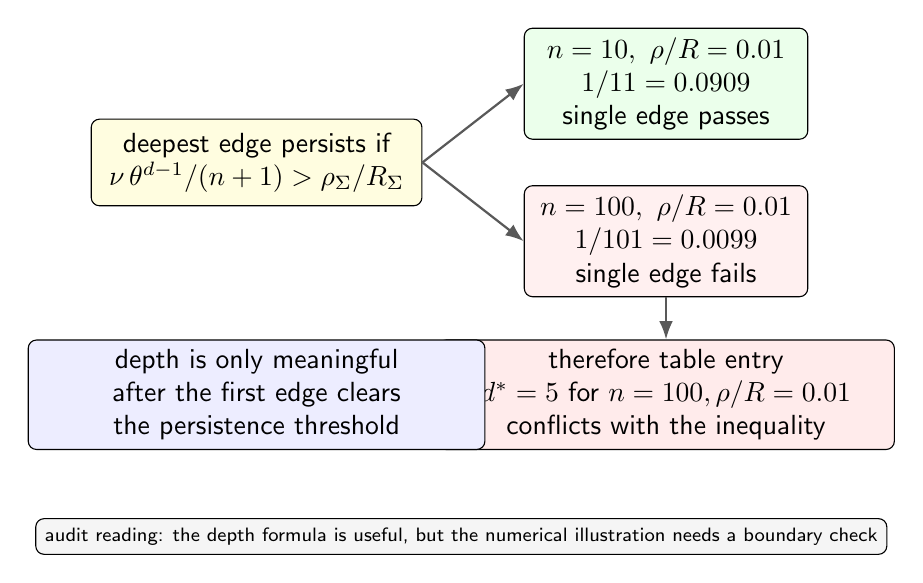
\begin{tikzpicture}[
  font=\sffamily,
  box/.style={draw, rounded corners=3pt, align=center, minimum width=42mm, minimum height=11mm, fill=white},
  note/.style={align=center, font=\sffamily\scriptsize},
  arrow/.style={-Latex, thick, draw=black!65},
  fail/.style={draw, rounded corners=3pt, align=center, minimum width=36mm, minimum height=10mm, fill=red!6},
  ok/.style={draw, rounded corners=3pt, align=center, minimum width=36mm, minimum height=10mm, fill=green!8}
]

\node[box, fill=yellow!12] (ineq) at (0,1.5)
  {deepest edge persists if\\$\nu\,\theta^{d-1}/(n+1) > \rho_\Sigma/R_\Sigma$};

\node[ok] (row1) at (5.2,2.5)
  {$n=10,\ \rho/R=0.01$\\$1/11=0.0909$\\single edge passes};
\node[fail] (row2) at (5.2,0.5)
  {$n=100,\ \rho/R=0.01$\\$1/101=0.0099$\\single edge fails};

\draw[arrow] (ineq.east) -- (row1.west);
\draw[arrow] (ineq.east) -- (row2.west);

\node[box, fill=red!8, minimum width=58mm] (table) at (5.2,-1.45)
  {therefore table entry\\$d^\ast=5$ for $n=100,\rho/R=0.01$\\conflicts with the inequality};
\draw[arrow] (row2.south) -- (table.north);

\node[box, fill=blue!7, minimum width=58mm] at (0,-1.45)
  {depth is only meaningful\\after the first edge clears\\the persistence threshold};

\node[note, fill=gray!8, draw, rounded corners=3pt, minimum width=86mm] at (2.6,-3.25)
  {audit reading: the depth formula is useful, but the numerical illustration needs a boundary check};

\end{tikzpicture}
\end{document}
